\cleardoublepage
% \newpage
% \thispagestyle{empty}
% \mbox{}

\chapter{Optimización del rendimiento de OmpSs sobre arquitecturas asimétricas}
\label{ch:chapter4}

%\section{Descripción de la estrategia de optimización}
%
%\section{BLIS}
%
%\subsection{Adaptación de BLIS a arquitecturas asimétricas}
%
%\section{Combinación de BLIS asimétrico con OmpSs}
%
\section{Planteamiento y objetivos generales}

Este capítulo presenta un nuevo acercamiento hacia la utilización de planificadores de tareas
no conscientes de la asimetría (en adelante nos referiremos a ellos como {\em convencionales})
sobre arquitecturas asimétricas, explotando toda la capacidad de cómputo de las mismas sin que
ello suponga una adaptación específica de las políticas de planificación de los mismos. Para ello,
se aprovechan implementaciones de tareas conscientes de la asimetría, abstrayendo al runtime de
dicha característica. 

En primer lugar, se llevará a cabo una evaluación inicial de la implementación por bloques de 
la factorización de Cholesky mostrada anteriormente en las Figuras~\ref{lst:chol} y \ref{lst:chol_tasks},
utilizando el planificador convencional de OmpSs y una versión secuencial de BLIS. Las observaciones de
dicho estudio servirán como base para la propuesta de solución introducida, consistente en el uso de
un planificador convencional enlazado con una versión asimétrica de BLIS. Finalmente, se comparan los
resultados obtenidos con los de los mismos códigos utilizando una versión de OmpSs consciente de la
arquitectura; finalmente, estos resultados son analizados en detalle a través de trazas de ejecución.

\subsection{Evaluación de runtimes convencionales en AMPs}
\label{subsec:conv_eval}

La Figura~\ref{fig:ompss_blis_oversubscription} muestra el rendimiento, en términos de GFLOPS (miles de millones de
operaciones en coma flotante por segundo), mostrado por el runtime convencional de OmpSs para la factorización
de Cholesky, variando el número de \wts entre~1 y~8 sobre la plataforma asimétrica \odroid; en el 
experimento, se delega la asignación de \wts a núcleos al planificador del sistema operativo. En otras palabras,
se está utilizando una versión no consciente de la asimetría del planificador de tareas en OmpSs.
Para este experimento, se ha evaluado un rango lo suficientemente amplio de tamaños de bloque 
({\tt b} en el código de la Figura~\ref{lst:chol}), aunque por simplicidad se reporta únicamente los
resultados obtenidos para el valor de {\tt b} que optimiza el ratio de GFLOPS para cada dimensión
del problema\footnote{En este capítulo, todos los experimentos se han realizado utilizando doble precisión.}.

\begin{figure}
\centering
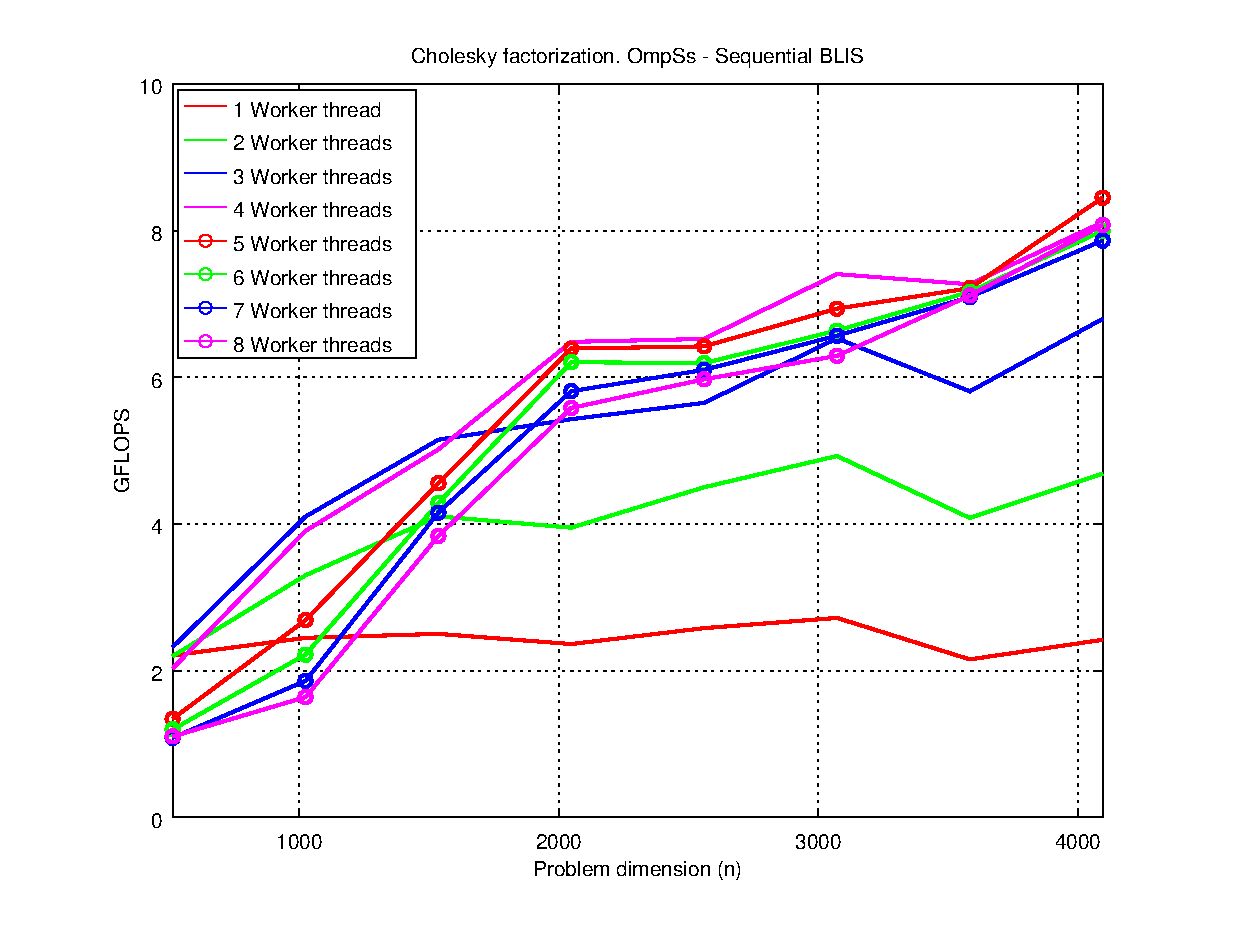
\includegraphics[width=0.70\textwidth]{Plots/Orig_runtime/plot_1to8_th}
\caption{Rendimiento de la factorización de Cholesky utilizando el runtime OmpSs convencional y una implementación secuencial
	de BLIS sobre el SoC Exynos 5422.}
\label{fig:ompss_blis_oversubscription}
\end{figure}

%All the experiments hereafter employed {\sc ieee} double precision. Furthermore,
%we  ensured that the cores operate at the highest possible frequency by setting the appropriate {\em cpufreq} governor.
%The conventional runtime of OmpSs corresponds to release 15.06 of the Nanos++ runtime task scheduler.
%For this experiment, it is lined with the ``sequential'' implementation of BLIS in release 0.1.5.
%(For the experiments with the multi-threaded/asymmetric version of BLIS in the later sections, 
%we will use specialized versions of the codes in~\cite{asymBLIS} for slow+fast VCs.)

Los resultados experimentales revelan un incremento en el rendimiento a medida que el número de \wts aumenta entre~1 y~4,
casos en los que el planificador del sistema operativo asigna su ejecución a los núcleos rápidos (Cortex-A15) disponibles.
Sin embargo, cuando el número de \wts excede la cantidad de núcleos rápidos, el sistema operativo se ve forzado a asignar
\wts a núcleos lentos (Cortex-A7), en cuyo caso el aumento en prestaciones desaparece, e incluso éstas disminuyen drásticamente 
a medida que el número de \wts aumenta. La principal causa de este decremento en las prestaciones es el desequilibrio de carga,
ya que tareas con granularidad uniforme, posiblemente pertenecientes al camino crítico, son asignadas a núcleos lentos.

Este experimento revela la principal motivación por la que es necesario un planificador de tareas consciente de la
arquitectura y adaptado a ella~\cite{OmpSsbigLITTLE}. Sin embargo, en el presente capítulo, se desarrollará un enfoque alternativo
a la hora de explotar la asimetría de la arquitectura subyacente: se utilizará un planificador de tareas convencional en combinación
con una biblioteca asimétrica para la ejecución de tareas, como se describe a continuación.

\section{Combinación de runtimes convencionales con bibliotecas asimétricas}

\subsection{Visión general de la propuesta}

La propuesta de operación introducida en el presente capítulo opera bajo el modelo GTS, pero está en cierto modo 
inspirada en el modelo CPUM (véase Sección~\ref{sec:models}). Más concretamente, el objetivo es que el planificador
de tareas considere la arquitectura \odroid (por ejemplo) como una arquitectura verdaderamente simétrica, formada por 
cuatro VCs (núcleos virtuales, o {\em Virtual Cores}), cada uno de ellos compuesto por un núcleo rápido y un núcleo
lento. Para ello, a diferencia del modelo CPUM, {\em ambos} núcleos físicos dentro de cada VC se mantendrán activos y 
colaborarán en la ejecución de una determinada tarea. Así, la propuesta explota dos niveles de concurrencia: el {\em paralelismo
a nivel de tareas} es extraído por el planificador para asignar tareas a cada uno de los cuatro VCs idénticos disponibles en
el sistema, e internamente, cada tarea/kernel divide su carga de forma correcta para exponer {\em paralelismo a nivel de datos}, 
distribuyendo la carga de trabajo entre los dos núcleos físicos asimétricos dentro del VC que está a cargo de la ejecución
de dicha tarea.

Esta solución requiere únicamente un planificador de tareas convencional (es decir, no consciente de la asimetría de la arquitectura, o lo
que es lo mismo, orientado a arquitecturas SMT), como por ejemplo el planificador de tareas convencional proporcionado por OmpSs, donde, 
en lugar de crear un \wt\ por núcleo físico del sistema, se sigue una filosofía similar a la propuesta por el modelo CPUM, creando 
{\em un único worker thread por VC}. Internamente, cuando una tarea es elegida para ser ejecutada por un \wt disponible, dicha tarea
se ejecutará, de forma ya no secuencial, sino paralela sobre cada uno de los núcleos que componen el VC, explotando, en este caso,
la asimetría interna de dicha abstracción. Por ejemplo, en el caso de \odroid, equipada con cuatro núcleos rápidos y cuatro lentos, 
la propuesta desarrollada desplegará únicamente cuatro \wts; para cualquier tarea básica o kernel de álgebra lineal a ejecutar, dicha
rutina explotará la asimetría internamente, siempre bajo la condición de que existe una implementación de la misma optimizada para
este tipo de paralelismo asimétrico.

Siguiendo esta idea, la arquitectura expuesta al planificador de tareas es completamente {\em simétrica}, y los kernels en BLIS
(o en cualquier otra biblioteca utilizada para la ejecución de las tareas) configuran una ``caja negra'' que abstrae del carácter
asimétrico al planificador.

En resumen, si en una configuración convencional el núcleo es el recurso mínimo de computación para el planificador de tareas,
y éstas son totalmente secuenciales, en la solución propuesta el VC es el recurso básico de computación de cara al planificador,
mientras que la implementación de las tareas pasa a ser no sólo paralela, sino adaptada para la correcta explotación del paralelismo
existente dentro de cada VC.

\subsection{Comparación y ventajas frente a otras alternativas}


%Provided an underlying asymmetry-aware library is available to the developer, it is possible to combine this 
%with an existing conventional runtime task scheduler in order to exploit the underlying architecture. 
%In the enhanced version of OmpSs in~\cite{OmpSsbigLITTLE}, tasks were actually invocations to a {\em sequential} 
%library implementation, and asymmetry was exploited via sophisticated scheduling policies specially designed for asymmetric architectures. 
%Following our new approach, asymmetry is exploited at the library level, not at the runtime level. 
%To accommodate this, tasks are cast in terms of 
%invocations to a multi-threaded asymmetry-aware library (in our case, BLIS). 

La solución desarrollada reúne un conjunto de ventajas de cara al desarrollador:

\begin{itemize}
\item El planificador de tareas no es consciente de la asimetría, por lo que cualquier versión convencional 
      del mismo podrá trabajar sobre este tipo de sistemas sin modificaciones específicas. 
\item Cualquier política de planificación (por ejemplo, {\em work stealing}, planificación consciente de la localidad de datos,
      implementación de caches por software, \ldots) ya desarrollada para arquitecturas simétricas, o cualquier futura mejora,
      tendrá también un impacto directo en el rendimiento sobre el sistema asimétrico.
\item Cualquier mejora en la implementación de las bibliotecas asimétricas subyacentes (por ejemplo, BLIS) tendrá un impacto directo
      sobre el AMP. Esta observación se aplica a arquitecturas con distinto número de núcleos lentos/rápidos dentro del VC, ratios
      en las frecuencias de funcionamiento, o incluso ante la introducción de más niveles de asimetría (esto es, núcleos con rendimiento
      intermedio).
\end{itemize}

Obviamente, existe una dificultad adicional intrínseca a la solución propuesta, y que se convierte en un requisito fundamental de cara
a su viabilidad: debe existir, necesariamente, una versión consciente de la asimetría para cada tarea a ejecutar (por ejemplo, una implementación
completa de las rutinas BLAS). En el ámbito del álgebra lineal densa, este requisito se cumple a través de la versión asimétrica de BLIS, aunque
en otros ámbitos, el desarrollo específico de este tipo de implementaciones es todavía escaso.

\subsection{Requisitos a nivel de tarea en el ámbito del álgebra lineal}

\comentario{Hay que reescribir esta sección}

Por último, cabe destacar que son necesarios ciertos requisitos adicionales en la implementación multihebra de BLIS
que opera sobre el modelo propuesto. Considérese el kernel \gemm y la descripción de alto nivel proporcionada en la Figura~\ref{lst:gemm}. 
Como se ha descrito anteriormente, resulta necesario distribuir el espacio de iteraciones de alguno de los bucles entre los dos tipos de núcleos
que conforman un VC; siguiendo las directivas de paralelización descritas en~\cite{BLIS3}, se distinguen a continuación dos escenarios de reparto posibles:

\begin{itemize}
	\item En arquitecturas donde cada VC está compuesto por igual número de núcleos de cada tipo (por ejemplo, \odroid) \ldots

	\item En arquitecturas donde cada VC está compuesto por distinto número de núcleos de cada tipo (por ejemplo, \juno) \ldots

\end{itemize}

For our objective, we still have to distribute the iteration space between the Cortex-A15 and the Cortex-A7 but, since there is only one resource of each type per VC,
there is no need to partition the loops internal to the macro-kernel. 
Furthermore, we note that the optimal strides for Loop~1 are in practice quite
large ({\tt nc} is in the order of a few thousands for ARM big.LITTLE cores), while the optimal values for Loop~3 are much more reduced
({\tt mc} is 32 for the Cortex-A7 and 156 for the Cortex-A15). Therefore, we target Loop~3 in our data-parallel implementation of BLIS for
VCs, which we can expect to easily yield a proper workload balancing.

%That is, both the number of cores to use, and the distribution of those cores between the fast and slow processing units are transparent and 
%fully configurable by the user. 

\section{Resultados experimentales}

\subsection{Estudio experimental del tamaño de bloque óptimo}

En tiempo de ejecución, OmpSs descompone la rutina para la implementación de la factorización de Cholesky en una colección de tareas
que operan en submatrices (bloques) con una granularidad que viene definida por el tamaño de bloque {\tt b}, véase el código en la 
Figura~\ref{lst:chol}. Estas tareas típicamente se reducen a invocaciones a kernels elementales a nivel de BLAS (en nuestro caso,
BLIS) o LAPACK, véase el código proporcionado en la Figura~\ref{lst:chol_tasks}.  

\newcommand{\bopt}{b^{\mbox{\rm \scriptsize opt}}\xspace}

El primer paso en nuestra evaluación radica en proporcionar una estimación realista de la ganancia de rendimiento
potencial proporcionada por la solución propuesta (en caso de haberla). Un factor crítico desde este punto de vista es
el rango de tamaños de bloque que resultan óptimos para el runtime convencional de OmpSs ante una determinada operación
(en adelante $\bopt$). En particular, la eficiencia de la solución propuesta vendrá determinada por el rendimiento obtenido
por las implementaciones BLIS de cada una de las tareas que componen la operación, comparada con su implementación secuencial
equivalente para dimensiones del problema {\tt n} en el orden de dimensión $bopt$.

La Tabla~\ref{tab:optimal_bs_sym} muestra los tamaños de bloque óptimos $\bopt$ para la factorización de Cholesky y tamaños
de problema crecientes, utilizando el planificador OmpSs convencional enlazado con una versión secuencial de BLIS y un número
creciente de \wts entre~1 y~4. Obsérvese como, excepto para los menores tamaños de problema, los tamaños de bloque óptimos están
en el rango entre 192 y 448. Estos tamaños de bloque resultan óptimos al ofrecer un equilibrio entre el paralelismo a nivel de tareas
potencial y la eficiencia interna de las ejecuciones secuenciales de cada tarea individual.

\newcommand{\ra}[1]{\renewcommand{\arraystretch}{#1}}
\newcommand{\ca}[1]{\renewcommand{\tabcolsep}{#1}}

\ra{1.2}
\ca{2pt}

\begin{table}
	\centering
	\caption{Tamaños de bloque óptimos para la factorización de Cholesky utilizando el planificador convencional
	         de OmpSs y una implementación secuencial de BLIS sobre \odroid.}
	\label{tab:optimal_bs_sym}
{\scriptsize
\begin{tabular}{crrrrrrrrrrrrrrrr} 
\toprule
  & \phantom{a} & \multicolumn{14}{c}{Tamaño del problema ({\tt n})} \\ 
\cmidrule{3-17} 
  & \phantom{a} &     512 & 1,024 & 1,536 & 2,048 & 2,560 & 3,072 & 3,584 & 4,096 & 4,608 & 5,120 & 5,632 & 6,144 & 6,656 & 7,168 & 7,680 \\ \hline

{\sc 1 wt} & \phantom{a} &     192 & 384  & 320  & 448  & 448  & 448  & 384  & 320 & 320 & 448 & 448 & 448 & 448 & 384 & 448 \\ \hline
{\sc 2 wt} & \phantom{a} &     192 & 192  & 320  & 192  & 448  & 448  & 384  & 320 & 320 & 448 & 448 & 448 & 448 & 384 & 448 \\ \hline
{\sc 3 wt} & \phantom{a} &     128 & 192  & 320  & 192  & 384  & 448  & 320  & 320 & 320 & 448 & 448 & 448 & 448 & 384 & 448 \\ \hline
{\sc 4 wt} & \phantom{a} &     128 & 128  & 192  & 192  & 192  & 320  & 320  & 320 & 320 & 448 & 320 & 448 & 448 & 384 & 448 \\ \bottomrule
\end{tabular}
}
\end{table}

La principal conclusión extraída tras el análisis de los resultados es la siguiente: para elevar el rendimiento de un planificador
de tareas combinado con una versión asimétrica de BLIS, cada uno de los kernels que componen la operación implementados en dicha
versión asimétrica debe exhibir mayor rendimiento que las respectivas implementaciones secuenciales, para dimensiones de matrices 
que estén en el orden de los tamaños de bloque mostrados en la Tabla~\ref{tab:optimal_bs_sym}.  

La Figura~\ref{fig:cross_blis} muestra el rendimiento alcanzado para las tres rutinas básicas BLAS que componen la factorización
de Cholesky (\gemm, \syrk y \trsm) para el rango de dimensiones de interés sobre la plataforma \odroid.  
El experimento compara la versión secuencial de BLIS sobre un único núcleo Cortex-A15 con la versión asimétrica de BLIS
que combina un Cortex-A15 y un Cortex-A7. Es decir, compara la ejecución de las tareas que componen la factorización sobre un
único núcleo físico (rápido) y sobre un VC (combinando un núcleo rápido y otro lento).

En general, las tres rutinas BLAS muestran una tendencia similar: los kernels de la versión secuencial de BLIS
consiguen mejor rendimiento que sus respectivas implementaciones asimétricas para tamaños de problema pequeños (hasta
aproximadamente {\tt m}, {\tt n}, {\tt k } = 128); sin embargo, 
a partir de dicha dimensión, el uso de un núcleo lento comienza a hacer que el rendimiento mejore. 
El aspecto más importante radica en el hecho de que el punto de corte entre ambas curvas está en el rango (e incluso 
es típicamente menor) de $\bopt$, véase Tabla~\ref{tab:optimal_bs_sym}. 
Esto implica que la versión asimétrica de BLIS puede, potencialmente, mejorar el rendimiento general de la factorización, 
incluso usando un planificador de tareas convencional.
Además, la mejora en rendimiento aumenta con el tamaño de problema, estabilizándose para dimensiones alrededor de 
{\tt m}, {\tt n}, {\tt k } $\approx~400$. Dado que este valor está en el rango del tamaño de bloque óptimo para
la factorización de Cholesky, sobre esta arquitectura es esperable una mejora en el orden de 0.3--0.5 GFLOPS por núcleo lento
añadido.
%mimicking the behavior of the underlying BLIS.

\begin{figure}[t]
\centering
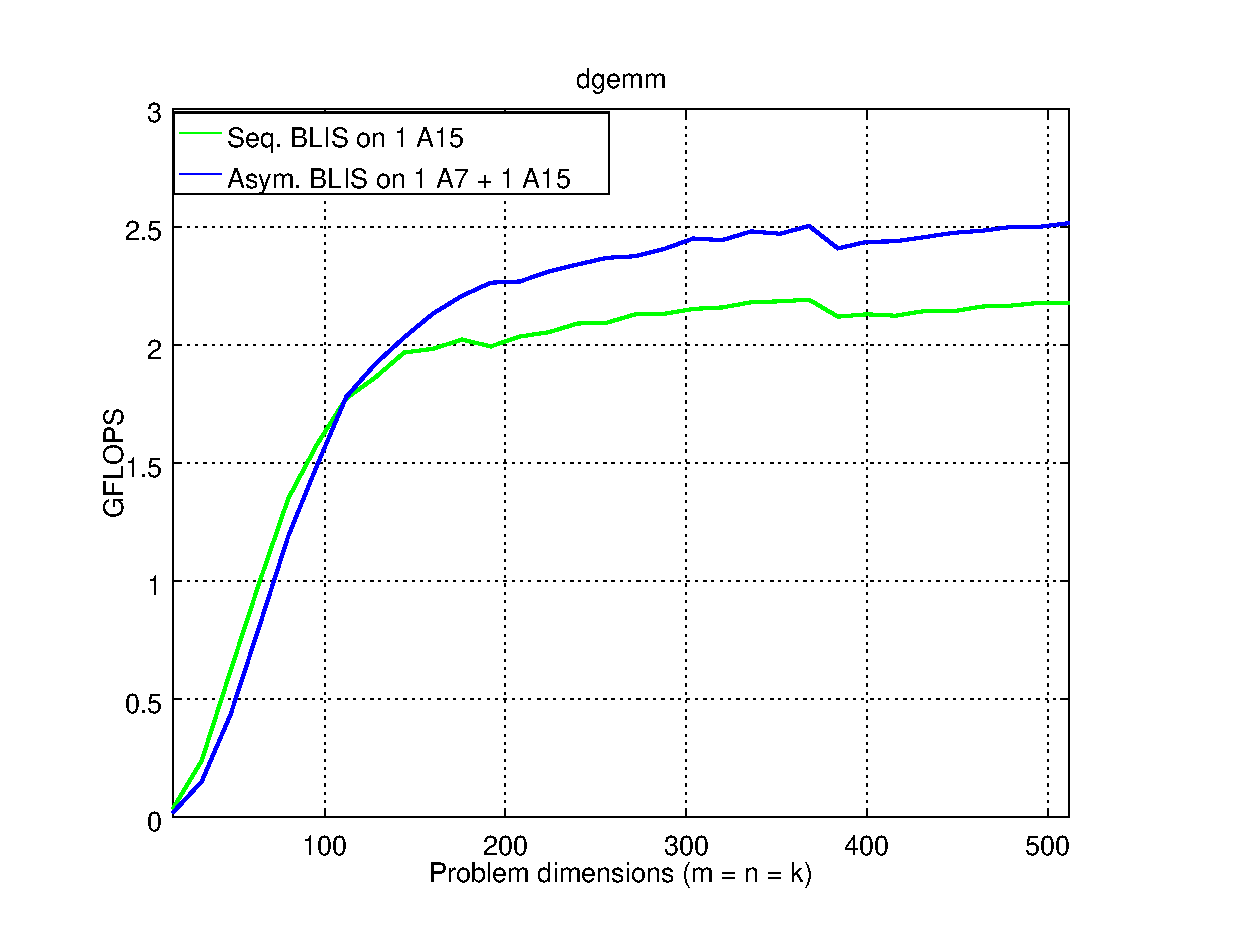
\includegraphics[width=0.49\textwidth]{Plots/BLIS_small/blis_dgemm_sym_asym}
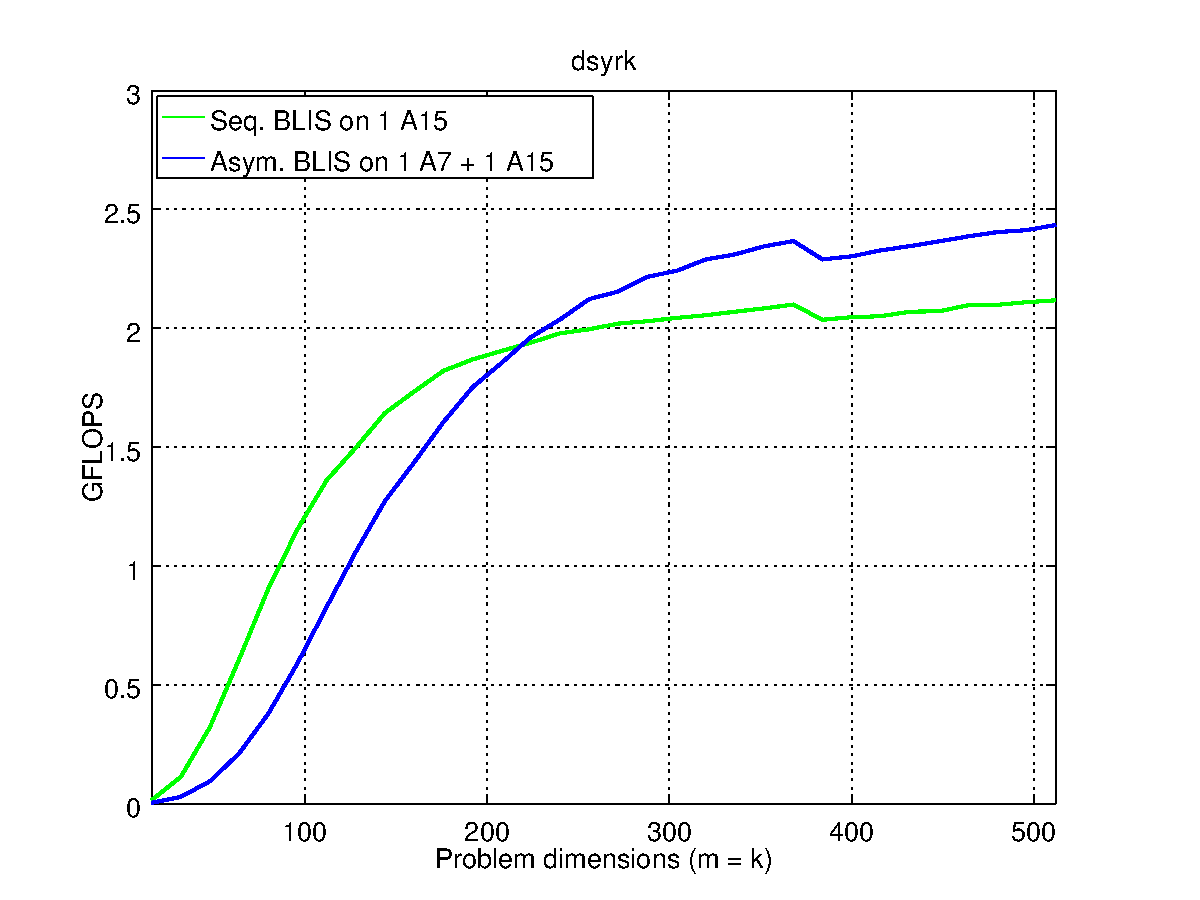
\includegraphics[width=0.49\textwidth]{Plots/BLIS_small/blis_dsyrk_sym_asym}
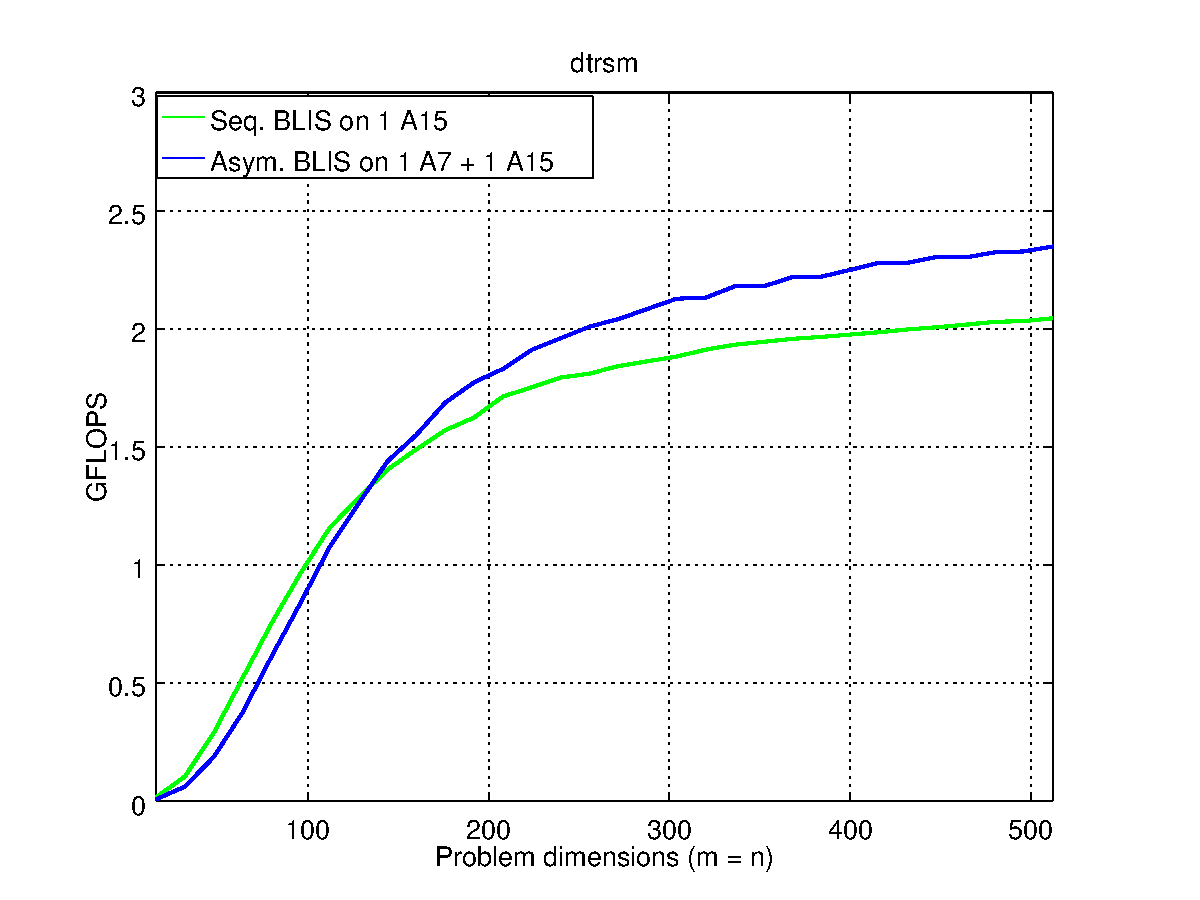
\includegraphics[width=0.49\textwidth]{Plots/BLIS_small/blis_dtrsm_sym_asym}
	\caption[Rendimiento de los kernels BLAS-3 en las implementaciones secuencial y asimétrica de BLIS.]{Rendimiento de los kernels BLAS-3 en las implementaciones secuencial y asimétrica de BLIS, utilizando, respectivamente
         un núcleo Cortex-A15 y un núcleo Cortex-A15 más un núcleo Cortex-A7 sobre \odroid.}
\label{fig:cross_blis}
\end{figure}


\subsection{Integración de BLIS asimétrico con un planificador de tareas convencional}

Con el fin de analizar los beneficios reales de la solución propuesta en términos de rendimiento, comparamos a continuación
el rendimiento del planificador OmpSs enlazado con {\em (a)} una versión secuencial de BLIS, y {\em (b)} con la versión asimétrica de BLIS. 
En todos los experimentos, los kernels BLIS en la primera configuración utilizaran exclusivamente un núcleo Cortex-A15, mientras
que en el segundo caso se utilizara un núcleo Cortex-A15 más un núcleo Cortex-A7 para la ejecución de las tareas.
%
La Figura~\ref{fig:ompss_blis} muestra los resultados obtenidos para ambas configuraciones, utilizando un número creciente
de \wts, entre~1 y~4. Por simplicidad, únicamente se reportan los resultados obtenidos considerando el tamaño de bloque óptimo
para cada tamaño de problema. En todos los casos, la solución basada en la utilización de una biblioteca asimétrica mejora
el rendimiento de la implementación secuencial para matrices relativamente grandes (típicamente con dimensiones {\tt n}~$>$~2,048)
mientras que, para tamaños de problema menores, el ratio de GFLOPS obtenido en ambos casos es similar. 
La razón de este comportamiento viene marcada por el tamaño de bloque óptimo reportado en la Tabla~\ref{tab:optimal_bs_sym}
y el rendimiento de BLIS mostrado en la Figura~\ref{fig:cross_blis}: para dicho rango de dimensiones de problema,
el tamaño óptimo de bloque es significativamente menor, y ambas implementaciones BLIS obtienen resultados de rendimiento similares.

\begin{figure}%[t]
\centering
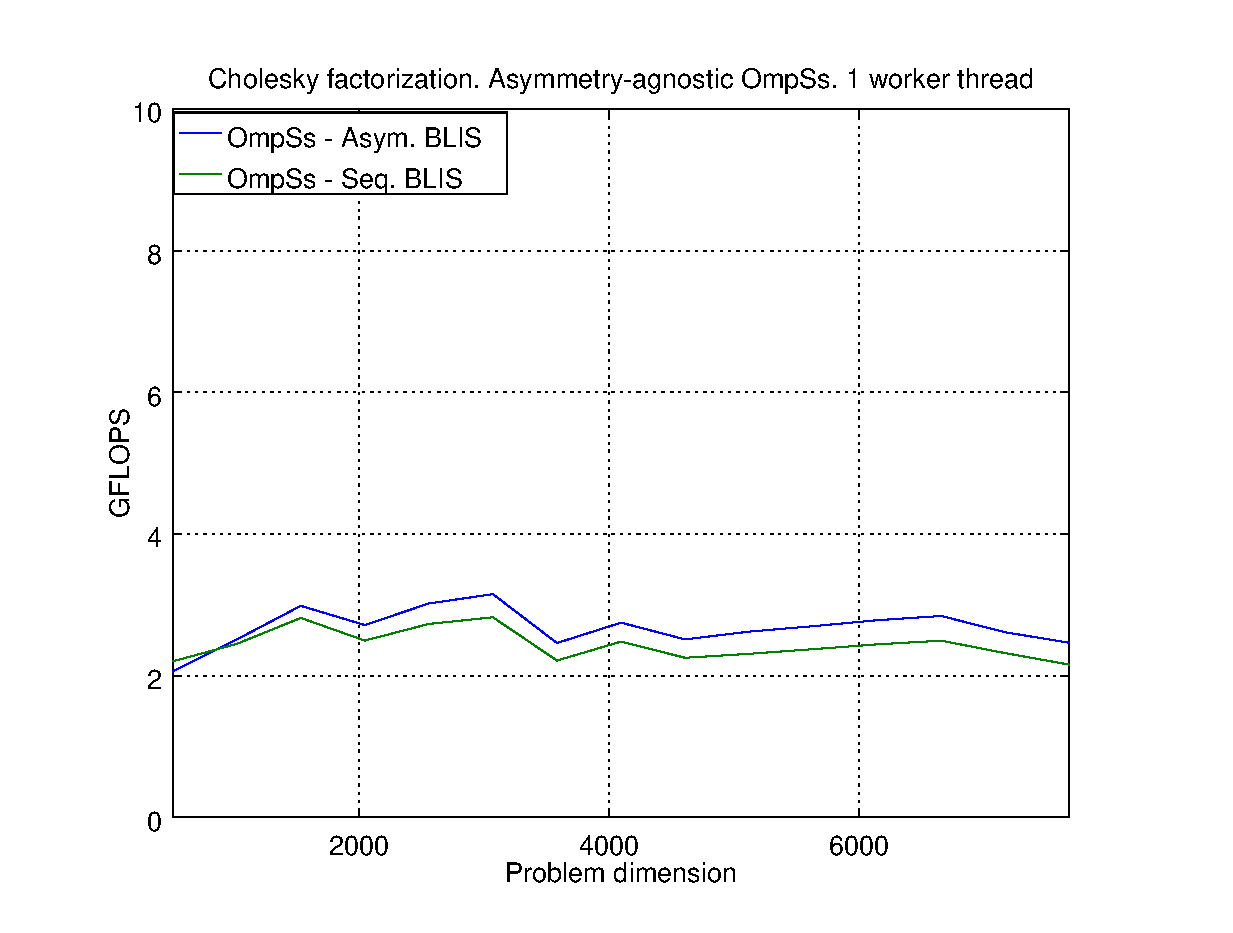
\includegraphics[width=0.49\textwidth]{Plots/Orig_runtime/plot_1_th}
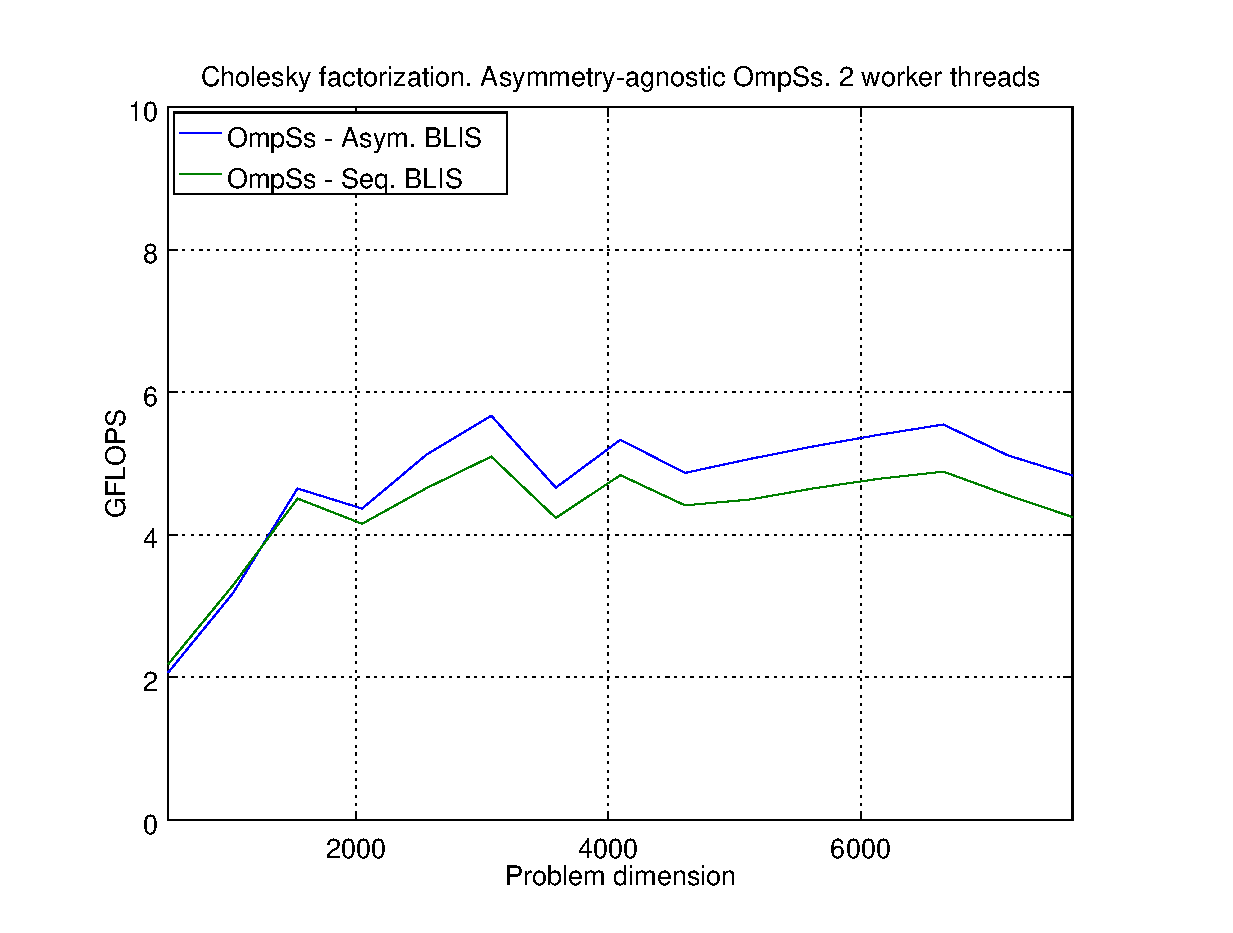
\includegraphics[width=0.49\textwidth]{Plots/Orig_runtime/plot_2_th}
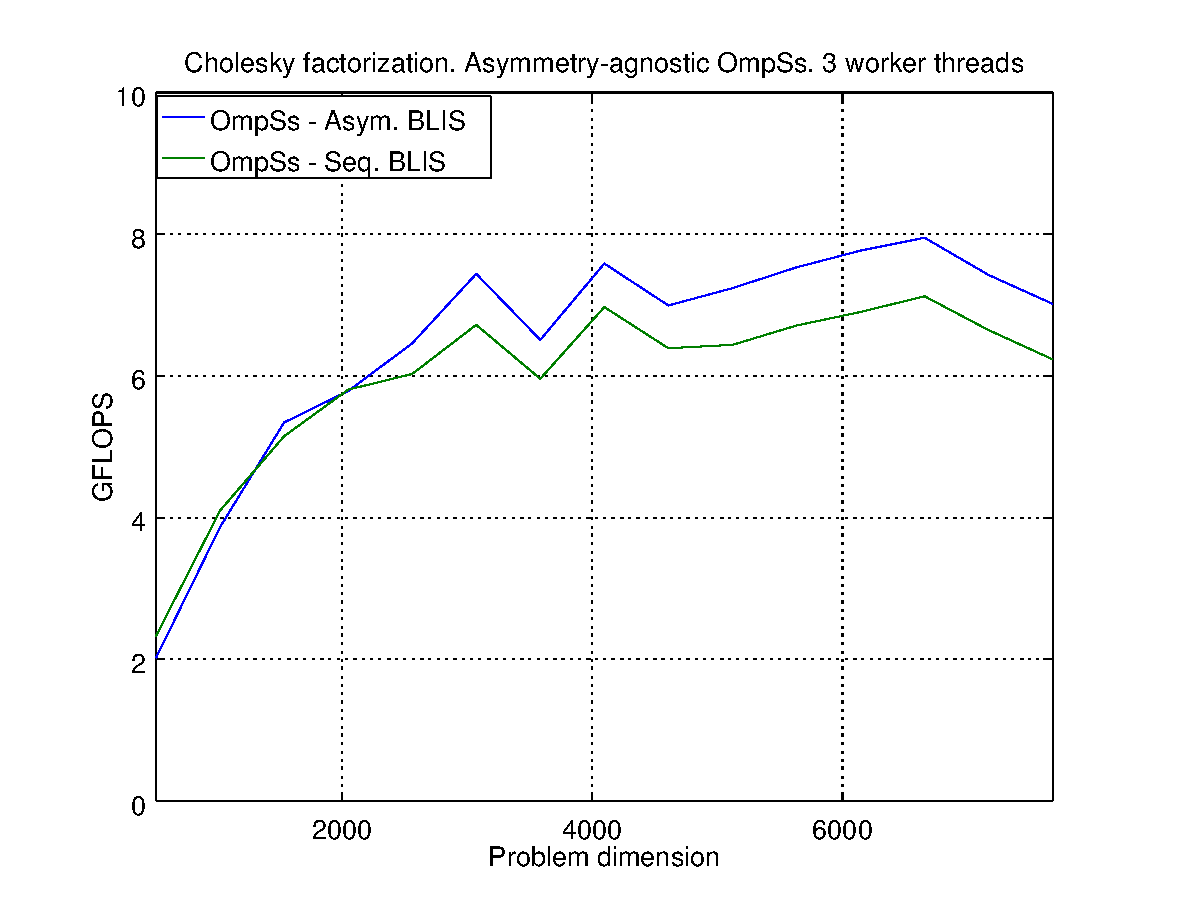
\includegraphics[width=0.49\textwidth]{Plots/Orig_runtime/plot_3_th}
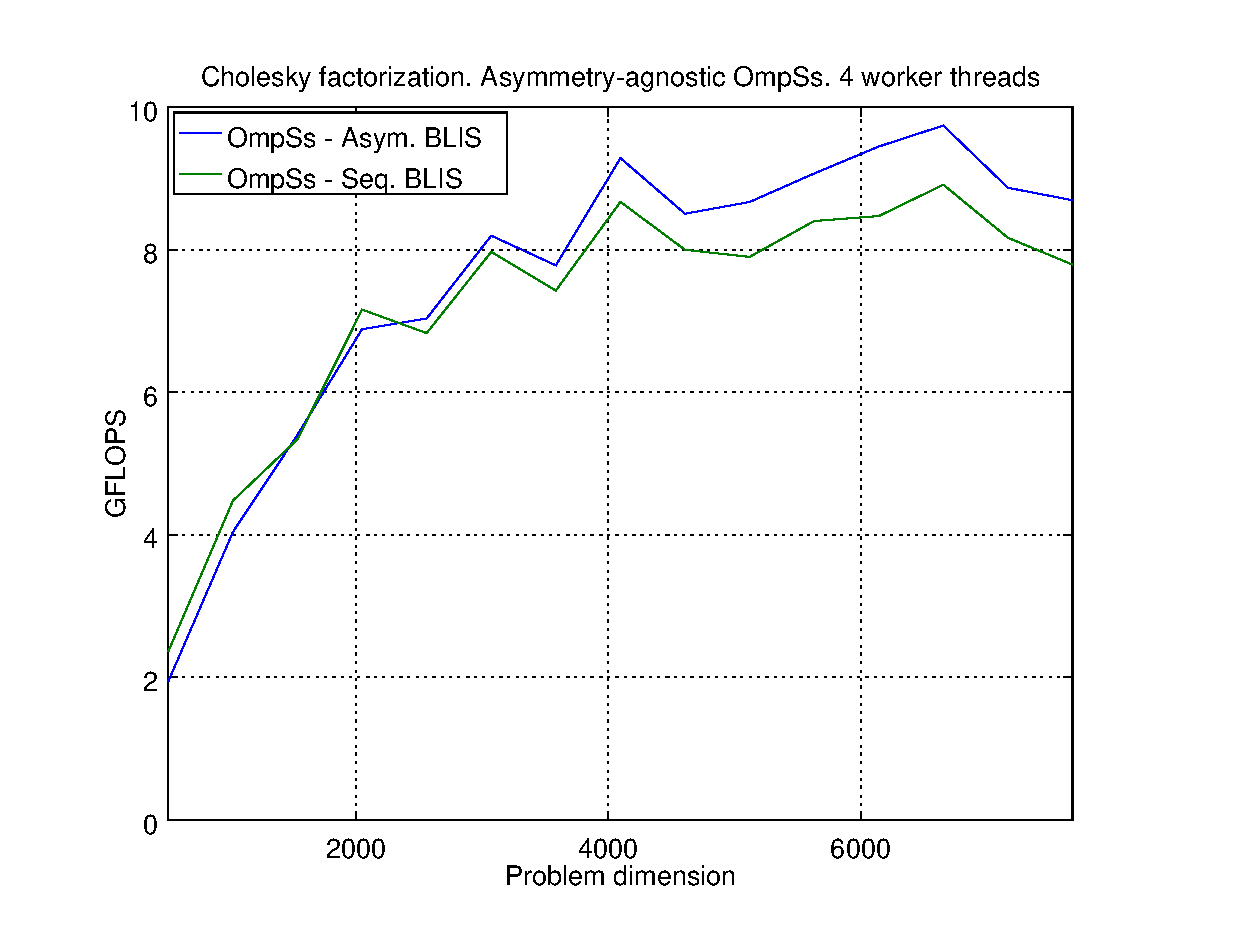
\includegraphics[width=0.49\textwidth]{Plots/Orig_runtime/plot_4_th}
\caption{Rendimiento de la factorización de Cholesky utilizando el planificador convencional de OmpSs, enlazado
         con la versión secuencial y asimétrica de BLIS.}
\label{fig:ompss_blis}
\end{figure}


%Table~\ref{tab:optimal_bs_sym}\ldots
%
%\begin{table}
	%\centering
	%\caption{Optimal block sizes for the Cholesky factorization using asymmetric BLIS.}
	%\label{tab:optimal_bs_asym}
	%\begin{tabular}{|c||c|c|c|c|c|c|c|c|c|c|c|c|c|c|c|}
		%\hline
		 %Th. &    512 & 1024 & 1536 & 2048 & 2560 & 3072 & 3584 & 4096 & 4608 & 5120 & 5632 & 6144 & 6656 & 7168 & 7680 \\ \hline \hline
		 %1   &    192 & 384 & 320 & 448 & 448 & 448 & 384 & 320 & 448 & 448 & 448 & 448 & 448 & 384 & 448 \\ \hline
		 %2   &    192 & 192 & 320 & 320 & 448 & 448 & 384 & 320 & 320 & 448 & 448 & 448 & 448 & 384 & 448 \\ \hline
		 %3   &    192 & 192 & 320 & 192 & 384 & 448 & 384 & 320 & 320 & 448 & 448 & 448 & 448 & 384 & 448 \\ \hline
		 %4   &    192 & 192 & 320 & 192 & 384 & 320 & 320 & 320 & 320 & 448 & 448 & 448 & 448 & 384 & 448 \\ \hline
	%\end{tabular}
%
%\end{table}

La diferencia cuantitativa en términos de rendimiento entre ambos enfoques se muestra
en las Tablas~\ref{tab:improvement_absolute} y~\ref{tab:improvement_percore}. 
La primera tabla muestra la diferencia absoluta en rendimiento, mientras que la segunda 
muestra la diferencia en rendimiento por cada núcleo lento (Cortex-A7) introducido en
el experimento. Consideremos, por ejemplo, el tamaño de problema {\tt n}~=~6,144. 
En este caso, el rendimiento mejora en 0.975 GFLOPS cuando se añaden los 4~núcleos lentos para 
dar soporte a los 4~núcleos Cortex-A15. Este hecho se traduce en una ganancia de rendimiento de
0.243 GFLOPS por core lento, ligeramente por debajo de la mejora que podría esperarse a partir de
los resultados experimentales observados en la anterior sección. Nótese, sin embargo, cómo el 
rendimiento por Cortex-A7 añadido se reduce desde 0.340~GFLOPS al añadir únicamente un núcleo,
hasta 0.243~GFLOPS, al utilizar los cuatro núcleos lentos.

\newcommand{\fg}[1]{\textcolor{ForestGreen}{#1}} % Verde
\newcommand{\br}[1]{\textcolor{BrickRed}{#1}} % Rojo

\begin{table}
	\centering
	\caption[Mejora de rendimiento absoluta (en GFLOPS) para la factorización de Cholesky utilizando
         el planificador OmpSs convencional enlazado con una versión asimétrica de BLIS.]{Mejora de rendimiento absoluta (en GFLOPS) para la factorización de Cholesky utilizando
         el planificador OmpSs convencional enlazado con una versión asimétrica de BLIS, con respecto
	 al mismo planificador enlazado con la versión secuencial de BLIS sobre \odroid.}
	 \label{tab:improvement_absolute}

%\begin{tabular}{|c||c|c|c|c|c|c|c|c|c|c|c|c|c|} 
   	%\hline
	%Th. &        512    & 1024       & 2048     & 2560     & 3072      & 4096     & 4608     & 5120    & 5632    & 6144     & 6656     & 7168     & 7680 \\ \hline \hline
	%1   &     -0.143    & 0.061      & 0.218    & 0.289    & 0.326     & 0.267    & 0.259    & 0.313   & 0.324   & 0.340    & 0.348    & 0.294    & 0.300    \\ \hline
	%2   &     -0.116    & -0.109     & 0.213    & 0.469    & 0.573     & 0.495    & 0.454    & 0.568   & 0.588   & 0.617    & 0.660    & 0.558    & 0.582    \\ \hline
	%3   &     -0.308    & -0.233     & -0.020   & 0.432    & 0.720     & 0.614    & 0.603    & 0.800   & 0.820   & 0.866    & 0.825    & 0.777    & 0.78    \\ \hline
	%4   &     -0.421    & -0.440     & -0.274   & 0.204    & 0.227     & 0.614    & 0.506    & 0.769   & 0.666   & 0.975    & 0.829    & 0.701    & 0.902    \\ \hline
%\end{tabular}
%%\end{table}

\ra{1.2}
\ca{2pt}

{\scriptsize
\begin{tabular}{crrrrrrrrrrrrr} 
   	\toprule
                 & \phantom{a} & \multicolumn{12}{c}{Dimensión del problema ({\tt n})} \\ 
\cmidrule{3-14} 
     & \phantom{a} &       512      & 1,024        & 2,048          & 2,560        & 3,072        & 4,096        & 4,608        & 5,120        & 5,632        & 6,144        & 6,656         & 7,680 \\ \hline 
{\sc 1 wt} & \phantom{a} &    \br{-0.143} & \fg{0.061}  & \fg{0.218}    & \fg{0.289}  & \fg{0.326}  & \fg{0.267}  & \fg{0.259}  & \fg{0.313}  & \fg{0.324}  & \fg{0.340}  & \fg{0.348}   & \fg{0.300} \\ \cline{3-14}
{\sc 2 wt} & \phantom{a} &    \br{-0.116} & \br{-0.109} & \fg{0.213}    & \fg{0.469}  & \fg{0.573}  & \fg{0.495}  & \fg{0.454}  & \fg{0.568}  & \fg{0.588}  & \fg{0.617}  & \fg{0.660}   & \fg{0.582} \\ \cline{3-14}
{\sc 3 wt} & \phantom{a} &    \br{-0.308} & \br{-0.233} & \br{-0.020}   & \fg{0.432}  & \fg{0.720}  & \fg{0.614}  & \fg{0.603}  & \fg{0.800}  & \fg{0.820}  & \fg{0.866}  & \fg{0.825}   & \fg{0.780} \\ \cline{3-14}
{\sc 4 wt} & \phantom{a} &    \br{-0.421} & \br{-0.440} & \br{-0.274}   & \fg{0.204}  & \fg{0.227}  & \fg{0.614}  & \fg{0.506}  & \fg{0.769}  & \fg{0.666}  & \fg{0.975}  & \fg{0.829}   & \fg{0.902} \\ \bottomrule
\end{tabular}
}
\end{table}


%\begin{table}
	%\centering
	%\caption{Performance improvement per introduced core (in GFLOPS) when using asymmetric BLIS combined with OmpSs for the Cholesky factorization.}
	%\label{tab:improvement_percore}
%
%\begin{tabular}{|c||c|c|c|c|c|c|c|c|c|c|c|c|c|} 
   	%\hline
	 %Th. &       512    & 1024     & 2048     & 2560     & 3072      & 4096     & 4608     & 5120    & 5632     & 6144     & 6656    & 7168     & 7680 \\ \hline \hline
	 %1   &    -0.143    & 0.061    & 0.218    & 0.289    & 0.326     & 0.267    & 0.259    & 0.313   & 0.324    & 0.340    & 0.348   & 0.294    & 0.300    \\ \hline
	 %2   &    -0.058    & -0.054   & 0.106    & 0.234    & 0.286     & 0.247    & 0.227    & 0.284   & 0.294    & 0.308    & 0.330   & 0.279    & 0.291    \\ \hline
	 %3   &    -0.102    & -0.077   & -0.006   & 0.144    & 0.240     & 0.204    & 0.201    & 0.266   & 0.273    & 0.288    & 0.275   & 0.259    & 0.261    \\ \hline
	 %4   &    -0.105    & -0.110   & -0.068   & 0.051    & 0.056     & 0.153    & 0.126    & 0.192   & 0.166    & 0.243    & 0.207   & 0.175    & 0.225    \\ \hline
%\end{tabular}
%
%\end{table}


\begin{table}
\centering
	\caption[Mejora de rendimiento por núcleo lento (en GFLOPS) para la factorización de Cholesky utilizando el planificador OmpSs convencional enlazado con una versión asimétrica de BLIS.]
	{Mejora de rendimiento por núcleo lento (en GFLOPS) para la factorización de Cholesky utilizando
         el planificador OmpSs convencional enlazado con una versión asimétrica de BLIS, con respecto
	 al mismo planificador enlazado con la versión secuencial de BLIS sobre \odroid.}
\label{tab:improvement_percore}

\ra{1.2}
\ca{2pt}
{\scriptsize
\begin{tabular}{crrrrrrrrrrrrr} 
   	\toprule
                 & \phantom{a} & \multicolumn{12}{c}{Dimensión del problema ({\tt n})} \\ 
\cmidrule{3-14} 
     & \phantom{a} &       512      & 1,024        & 2,048          & 2,560        & 3,072        & 4,096        & 4,608        & 5,120        & 5,632        & 6,144        & 6,656         & 7,680 \\ \hline 
	 {\sc 1 wt}    & \phantom{a} &    \br{-0.143} & \fg{0.061}  & \fg{0.218}  & \fg{0.289} & \fg{0.326}  & \fg{0.267} & \fg{0.259} & \fg{0.313} & \fg{0.324} & \fg{0.340} & \fg{0.348} & \fg{0.300}    \\ \cline{3-14}
	 {\sc 2 wt}    & \phantom{a} &    \br{-0.058} & \br{-0.054} & \fg{0.106}  & \fg{0.234} & \fg{0.286}  & \fg{0.247} & \fg{0.227} & \fg{0.284} & \fg{0.294} & \fg{0.308} & \fg{0.330} & \fg{0.291}    \\ \cline{3-14}
	 {\sc 3 wt}    & \phantom{a} &    \br{-0.102} & \br{-0.077} & \br{-0.006} & \fg{0.144} & \fg{0.240}  & \fg{0.204} & \fg{0.201} & \fg{0.266} & \fg{0.273} & \fg{0.288} & \fg{0.275} & \fg{0.261}    \\ \cline{3-14}
	 {\sc 4 wt}    & \phantom{a} &    \br{-0.105} & \br{-0.110} & \br{-0.068} & \fg{0.051} & \fg{0.056}  & \fg{0.153} & \fg{0.126} & \fg{0.192} & \fg{0.166} & \fg{0.243} & \fg{0.207} & \fg{0.225}    \\ \bottomrule
\end{tabular}
}

\end{table}

%% TABLAS ORIGINALES SIN SELECCIONAR COLUMNAS PARA QUE QUEPAN...
%\begin{table}
	%\centering
	%\caption{Absolute performance improvement (in GFLOPS) when using asymmetric BLIS combined with OmpSs for the Cholesky factorization.}
	%\label{tab:improvement_absolute}
%
%\begin{tabular}{|c||c|c|c|c|c|c|c|c|c|c|c|c|c|c|c|} 
   	%\hline
	%Th. &        512    & 1024     & 1536     & 2048     & 2560     & 3072     & 3584    & 4096     & 4608     & 5120    & 5632    & 6144     & 6656     & 7168     & 7680 \\ \hline \hline
	%1   &     -0.143    & 0.061    & 0.170    & 0.218    & 0.289    & 0.326    & 0.247   & 0.267    & 0.259    & 0.313   & 0.324   & 0.340    & 0.348    & 0.294    & 0.300    \\ \hline
	%2   &     -0.116    & -0.109   & 0.140    & 0.213    & 0.469    & 0.573    & 0.424   & 0.495    & 0.454    & 0.568   & 0.588   & 0.617    & 0.660    & 0.558    & 0.582    \\ \hline
	%3   &     -0.308    & -0.233   & 0.194    & -0.020   & 0.432    & 0.720    & 0.549   & 0.614    & 0.603    & 0.800   & 0.820   & 0.866    & 0.825    & 0.777    & 0.78    \\ \hline
	%4   &     -0.421    & -0.440   & 0.063    & -0.274   & 0.204    & 0.227    & 0.353   & 0.614    & 0.506    & 0.769   & 0.666   & 0.975    & 0.829    & 0.701    & 0.902    \\ \hline
%\end{tabular}
%\end{table}
%
%\begin{table}
	%\centering
	%\caption{Performance improvement per introduced core (in GFLOPS) when using asymmetric BLIS combined with OmpSs for the Cholesky factorization.}
	%\label{tab:improvement_percore}
%
%\begin{tabular}{|c||c|c|c|c|c|c|c|c|c|c|c|c|c|c|c|} 
   	%\hline
	 %Th. &       512    & 1024    & 1536    & 2048     & 2560     & 3072     & 3584    & 4096     & 4608     & 5120    & 5632     & 6144     & 6656    & 7168     & 7680 \\ \hline \hline
	 %1   &    -0.143    & 0.061   & 0.170   & 0.218    & 0.289    & 0.326    & 0.247   & 0.267    & 0.259    & 0.313   & 0.324    & 0.340    & 0.348   & 0.294    & 0.300    \\ \hline
	 %2   &    -0.058    & -0.054  & 0.070   & 0.106    & 0.234    & 0.286    & 0.212   & 0.247    & 0.227    & 0.284   & 0.294    & 0.308    & 0.330   & 0.279    & 0.291    \\ \hline
	 %3   &    -0.102    & -0.077  & 0.064   & -0.006   & 0.144    & 0.240    & 0.183   & 0.204    & 0.201    & 0.266   & 0.273    & 0.288    & 0.275   & 0.259    & 0.261    \\ \hline
	 %4   &    -0.105    & -0.110  & 0.015   & -0.068   & 0.051    & 0.056    & 0.088   & 0.153    & 0.126    & 0.192   & 0.166    & 0.243    & 0.207   & 0.175    & 0.225    \\ \hline
%\end{tabular}
%\end{table}

\subsection{Comparativa de rendimiento con un planificador consciente de la asimetría}
\label{sec:comparative}

El último conjunto de experimentos tiene como objetivo ofrecer una visión global de las ventajas en términos
de rendimiento de distintas configuraciones en la ejecución paralela a nivel de tareas de la factorización de
Cholesky utilizando el planificador de OmpSs. Más concretamente, se consideran a continuación las siguientes
alternativas:

\begin{enumerate}

	\item El planificador convencional OmpSs enlazado con una implementación secuencial de BLIS (``OmpSs - Seq. BLIS'').
	\item El planificador convencional OmpSs enlazado con la versión asimétrica de BLIS que considera el SoC como cuatro {\em núcleos virtuales (VC)} (``OmpSs - Asym. BLIS'').
	\item La versión consciente de la asimetría ({\em criticality-aware, o botlev}) de OmpSs, enlazada con la versión secuencial de BLIS (``Botlev-OmpS - Seq. BLIS''). 

\end{enumerate}

En las ejecuciones, se utilizan los cuatro núcleos Cortex-A15 y se evalúa el impacto de añadir núcleos 
Cortex-A7 a la configuración (entre 1 y 4) para el planificador Botlev.


La Figura~\ref{fig:comparative} muestra el rendimiento obtenido por cada una de las configuraciones
anteriormente descritas sobre la plataforma \odroid. Los resultados pueden ser analizados si se dividen 
en tres grandes grupos, atendiendo a la dimensión del problema:

\begin{itemize}
	\item Para matrices pequeñas ({\tt n}~=~512, 1,024), el planificador convencional utilizando exclusivamente cuatro núcleos rápidos (esto es,
		enlazado con la versión secuencial de BLIS para la ejecución de tareas) obtiene los mejores resultados en términos de rendimiento.
		Esta es una observación esperada y ya fue observada en la Figura~\ref{fig:ompss_blis}; la principal causa radica en el pequeño tamaño óptimo
		de bloque para este rango de dimensiones de problema, necesario para exponer el suficiente paralelismo a nivel de tareas. Esta necesidad invalida
		el uso de la implementación asimétrica de BLIS dado su bajo rendimiento sobre matrices de muy reducidas dimensiones; véase Figura~\ref{fig:cross_blis}. 
		Además, cabe destacar que el planificador OmpSs adaptado a la asimetría (Botlev) no obtiene ratios de rendimiento elevados para este rango de 
		dimensiones, independientemente del número de núcleos Cortex-A7 introducidos en el experimento.

 \item Para matrices de tamaño intermedio ({\tt n}~=~2,048, 4,096), la diferencia de rendimiento entre los diferentes enfoques se reduce.
	 La variante que utiliza la versión asimétrica de BLIS comienza a obtener mejores rendimientos que las implementaciones alternativas para
{\tt n}=4,096. Para este rango de dimensiones, Botlev-OmpSs es competitivo, y también obtiene mejores rendimientos que la configuración convencional.

 \item Para matrices de grandes dimensiones ({\tt n}~=~6,144, 7,680) la anterior tendencia se consolida, y ambos enfoques conscientes de la arquitectura muestran
	 ganancias de rendimiento considerables. Comparando ambos enfoques conscientes de la arquitectura, nuestra solución
obtiene mejor rendimiento, incluso considerando la utilización de todos los núcleos lentos para el planificador Botlev-OmpSs.

\end{itemize}

\begin{figure}
\centering
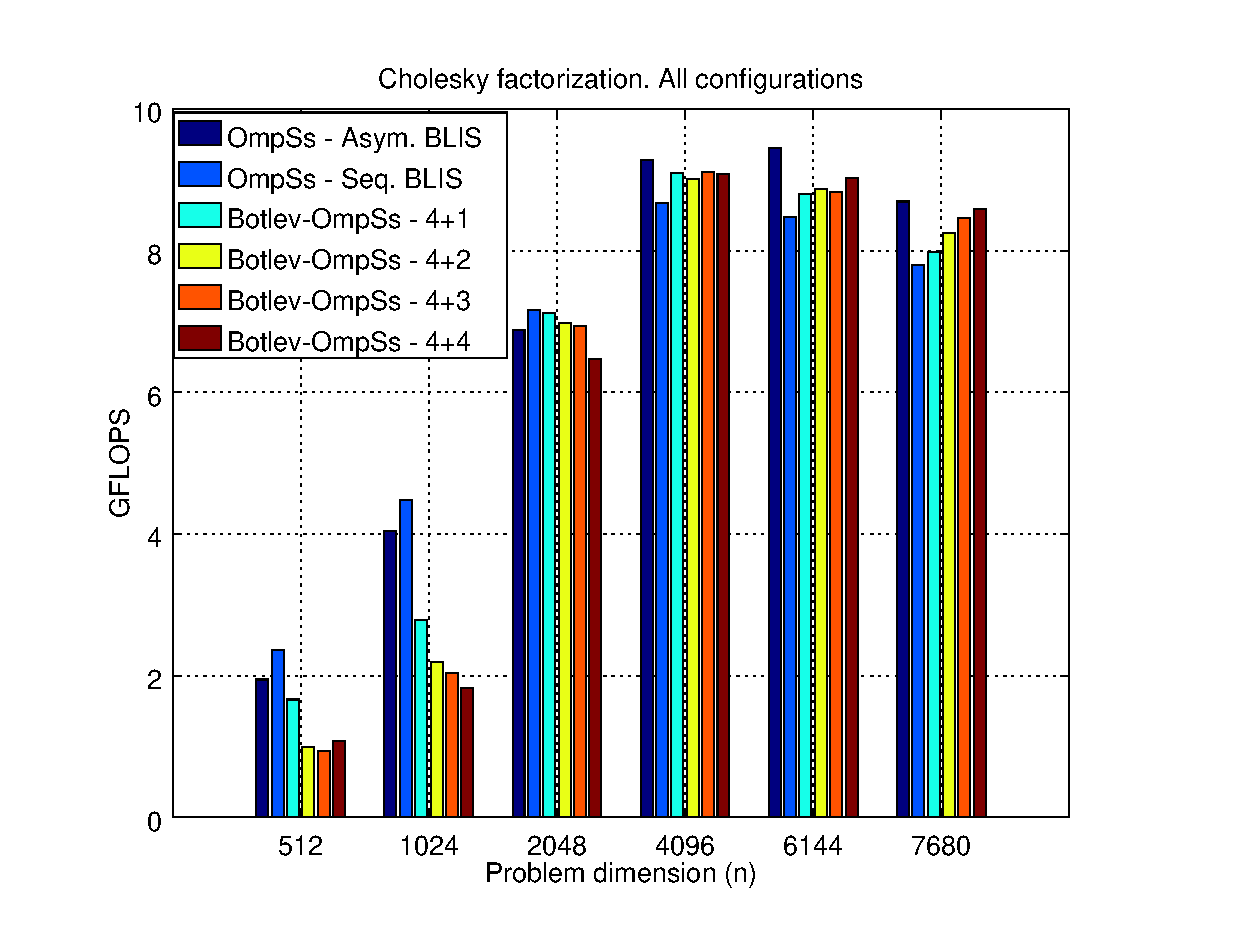
\includegraphics[width=0.70\textwidth]{Plots/Comparative/comparative}
	\caption[Rendimiento (en GFLOPS) para la factorización de Cholesky utilizando distintas implementaciones.]{Rendimiento (en GFLOPS) para la factorización de Cholesky utilizando 
el planificador convencional de OmpSs enlazado con la versión secuencial de BLIS, la implementación asimétrica de BLIS, y 
la implementación consciente de la arquitectura Botlev de OmpSs enlazado con la versión secuencial de BLIS sobre \odroid. 
Las etiquetas con la forma ``4+x'' indican una ejecución con 4~núcleos Cortex-A15 utilizando x núcleos Cortex-A7.}
\label{fig:comparative}
\end{figure}

En conclusión, nuestro enfoque para explotar la asimetría mejora tanto la portabilidad como la facilidad de
programación y desarrollo de planificadores de tareas, evitando el desarrollo de políticas específicas de planificación
conscientes de la asimetría. Además, el rendimiento obtenido es comparable con éstos para cualquier tamaño de problema; para
matrices de tamaño medio/grande, mejora además de forma sustancial el rendimiento conseguido por un planificador no consciente de la
asimetría.

\subsection{Análisis detallado de rendimiento}

A continuación, se proporcionan más detalles sobre el comportamiento, en términos de rendimiento, de cada una de las 
configuraciones anteriormente descritas. Las trazas de ejecución mostradas en esta sección han sido extraídas con la
herramienta de instrumentación {\tt Extrae}~\cite{Extrae} y visualizadas a través de la herramienta {\tt Paraver}~\cite{Paraver}.
Los resultados corresponden a un caso concreto de la factorización de Cholesky, con matriz de entrada de dimensión
{\tt n}~=~6,144 y tamaño de bloque {\tt b}~=~448.

\subsubsection{Visión general de la ejecución de tareas}

La Figura~\ref{fig:traces_tasks} muestra una traza completa de ejecución para cada configuración del planificador OmpSs. A grandes rasgos, es posible
extraer un conjunto de observaciones generales:

\begin{itemize}
\item Desde el punto de vista del tiempo total de ejecución, el planificador convencional de OmpSs combinado con una versión asimétrica
	de BLIS obtiene los mejores resultados, seguido por la implementación Botlev del planificador. Es necesario destacar que
		la versión no consciente de la asimetría de OmpSs, con 8 \wt y sin ninguna modificación adicional, obtiene los peores
		resultados con diferencia. En este caso, el desequilibrio de carga y los largos periodos de inactividad en la
		ejecución de tareas, especialmente a medida que el paralelismo de tareas disponible disminuye (en las últimas etapas
		de la ejecución) conllevan una penalización de rendimiento muy considerable.

\item Las marcas de inicio/finalización de cada tarea revelan que la versión asimétrica de BLIS (que utiliza los recursos combinados
	en cada VC) requiere menor tiempo de ejecución por tarea que las dos alternativas basadas en BLIS secuencial. Un efecto a observar
		es la lógica diferencia en rendimiento en la versión Botlev del planificador en la ejecución de las tareas sobre núcleos
		rápidos (\wts entre el 5 y el 8) y lentos (\wts entre el 1 y el 4). Este fenómeno no se observa en nuestra solución, ya
		que, para el planificador, cualquiera de los 4 \wts disponibles observa unidades de procesamiento (VCs) homogéneos.

\item El planificador Botlev-OmpSs incluye políticas complejas de planificación que incluyen el tratamiento de prioridades,
	avanzando la ejecución de tareas en el camino cŕitico y, cuando sea posible, asignando éstas a núcleos rápidos (véanse,
		por ejemplo, las tareas correspondientes a factorizaciones de los bloques diagonales, coloreadas en amarillo). Esta
		política induce una planificación más compactadurante las primeras fases de la ejecución paralela, pero 
		con mayores problemas a medida que el grado de concurrencia disminuye (en las últimas iteraciones de la 
		factorización). Aunque es posible, no se ha activado este tipo de gestión de prioridades en la versión convencional
		de OmpSs utilizada en el resto de experimentos, y su interacción con una implementación asimétrica de las tareas
		se plantea como trabajo futuro.
\end{itemize}


\begin{figure}%[t]
\centering
	\begin{subfigure}{\textwidth}
   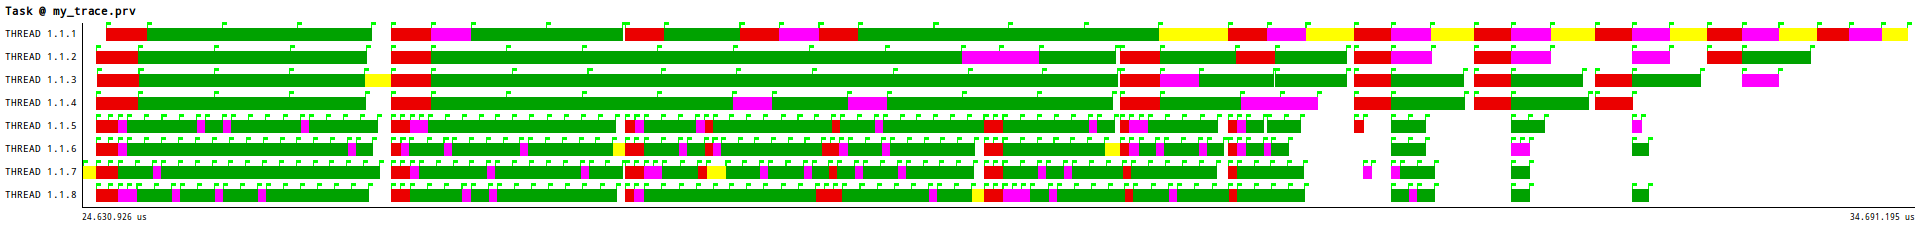
\includegraphics[width=\textwidth]{Plots/Traces/sym_8cores_tasks.png}
		\caption{OmpSs - BLIS secuencial (8 worker threads)} 
	\end{subfigure}
	\begin{subfigure}{\textwidth}
   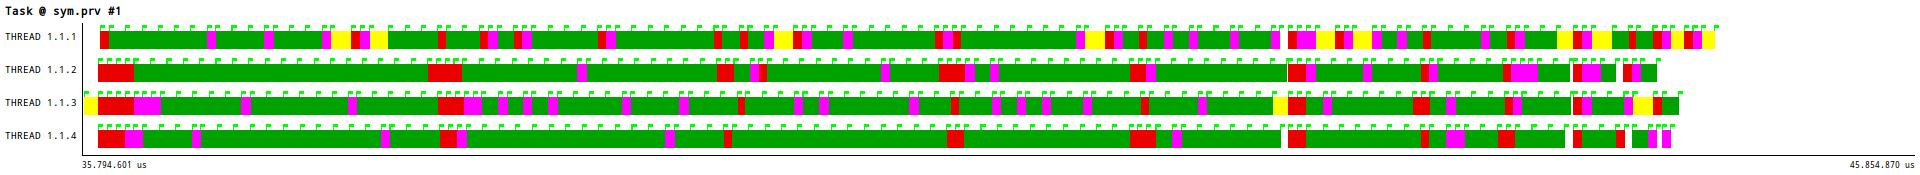
\includegraphics[width=\textwidth]{Plots/Traces/sym_tasks.png}
 \caption{OmpSs - BLIS secuencial (4 worker threads)} 
	\end{subfigure}
	\begin{subfigure}{\textwidth}
   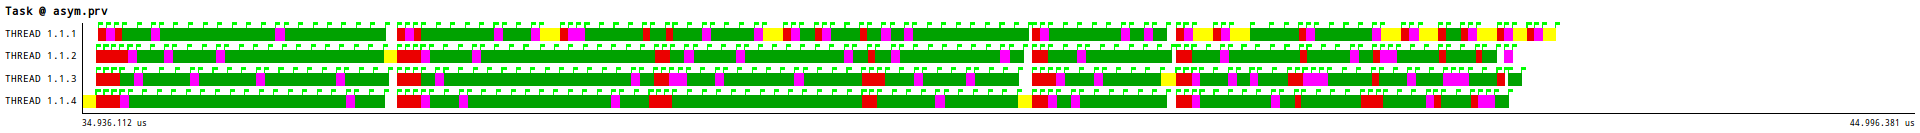
\includegraphics[width=\textwidth]{Plots/Traces/asym_tasks.png}
		\caption{OmpSs - BLIS asimétrico (4 worker threads)}
	\end{subfigure}
	\begin{subfigure}{\textwidth}
   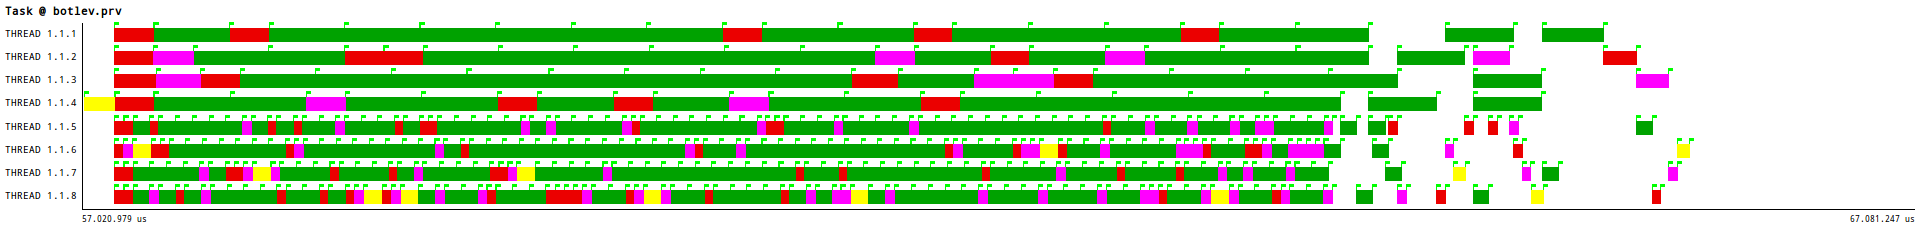
\includegraphics[width=\textwidth]{Plots/Traces/botlev_tasks.png}
		\caption{Botlev-OmpSs - BLIS secuencial (8 worker threads, 4+4)}
	\end{subfigure}
	\caption[Trazas de ejecución para las tres configuraciones estudiadas en la factorización de Cholesky ({\tt n}~=~6,144, {\tt b}~=~448).]
	{Trazas de ejecución para las tres configuraciones estudiadas en la factorización de Cholesky ({\tt n}~=~6,144, 
{\tt b}~=~448). 
La línea de tiempo en cada fila recoge las tareas ejecutadas por un único \wt.
Las tareas se han coloreado siguiendo la convención de la Figura~\ref{fig:dag};
las fases coloreadas en color blanco representan etapas sin actividad. Las marcas en color
	verde denotan puntos de inicialización de la ejecución de cada tarea.
}
\label{fig:traces_tasks}
\end{figure}


Se proporciona a continuación un análisis cuantitativo de la duración temporal de las tareas y un estudio
más detallado de la estrategia de planificación integrada en cada configuración.

\subsubsection{Duración de las tareas}
 
La Tabla~\ref{tab:2dp_tasks} muestra el tiempo medio de ejecución por tipo de tarea para cada \wt.
Los resultados muestran como el tiempo de ejecución para cada tipo de tarea es considerablemente menor
en la versión asimétrica de BLIS que en las alternativas basadas en ejecuciones secuenciales de las
tareas. La única excepción es la factorización de los bloques diagonales (rutina {\tt dpotrf}), ya que
se trata de una rutina perteneciente a LAPACK, y por tanto no disponible en BLIS y no paralelizada de forma
consciente de la asimetría). Inspeccionando la duración de las tareas en la configuración Botlev-OmpSs, 
se observa una notable diferencia en función del tipo de núcleo sobre el que el planificador mapea las tareas. Por
ejemplo, el tiempo medio de ejecución para {\tt dgemm} varía entre más de 400~ms en un núcleo lento, hasta prácticamente
90~ms en un núcleo rápido. Este comportamiento se reproduce para todos los tipos de tareas.

Para ilustrar más claramente estas observaciones, la Figura~\ref{fig:traces_task_duration} representa un histograma
detallado de los tiempos de ejecución para las distintas instancias de la tarea {\tt dgemm} durante la ejecución
paralela. Cada casilla corresponde al número de tareas con un tiempo de ejecución dado, mientras que las filas corresponden
a cada \wt en ejecución.
Comparando las configuraciones que utilizan planificadores convencionales (trazas (a) y (b)),
existe una clara desviación en el tiempo medio de ejecución hacia mayores rendimientos al utilizar
BLIS asimétrico, esto es, el tiempo medio de ejecución de una tarea es claramente menor en este caso. El histograma para Botlev (traza (c))
muestra dos zonas diferenciadas, que corresponden a tareas ejecutadas sobre núcleos rápidos y núcleos lentos, respectivamente. Nótese que
las tareas ejecutadas sobre núcleos rápidos obtienen el mismo rendimiento que las equivalentes en una configuración convencional
usando BLIS secuencial. Se ha observado un comportamiento similar para el resto de tareas BLAS ejecutadas durante el experimento.

\begin{figure}%[t]
\centering
	\begin{subfigure}{\textwidth}
   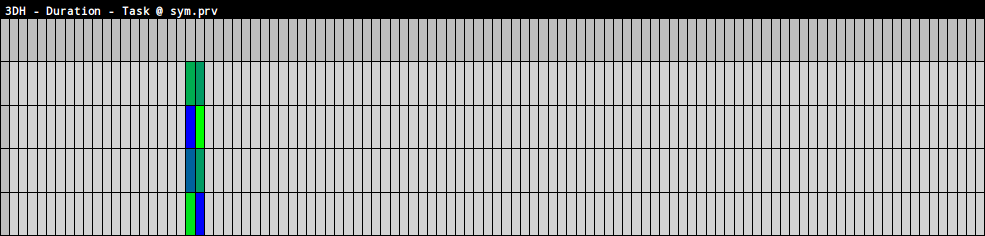
\includegraphics[width=\textwidth]{Plots/Traces/sym_task_duration_histogram.png}
 \caption{OmpSs + BLIS simétrico.}
	\end{subfigure}
	\begin{subfigure}{\textwidth}
   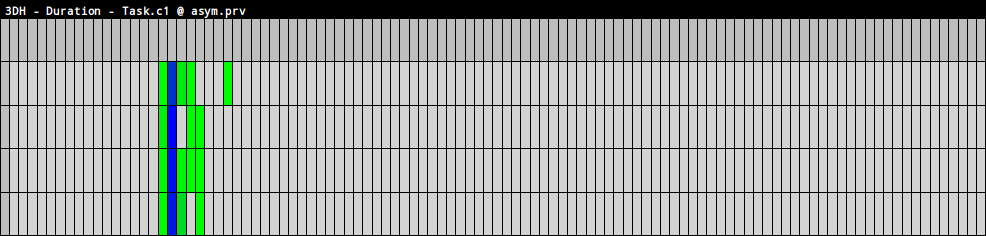
\includegraphics[width=\textwidth]{Plots/Traces/asym_task_duration_histogram.png}
		\caption{OmpSs + BLIS asimétrico.}
	\end{subfigure}
	\begin{subfigure}{\textwidth}
   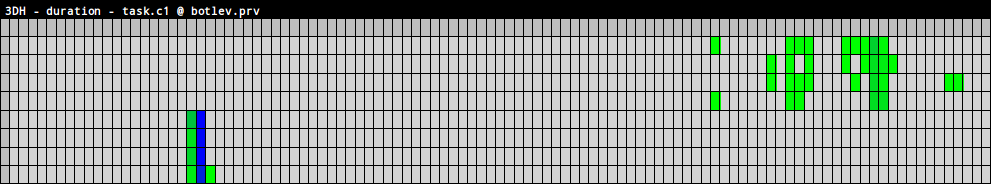
\includegraphics[width=\textwidth]{Plots/Traces/botlev_task_duration_histogram.png}
 \caption{Botlev-OmpSs - 4+4 hebras.}
	\end{subfigure}
	\caption[Histograma de duración de tareas para la tarea {\tt dgemm} sobre las tres configuraciones de planificador.]{Histograma de duración de tareas para la tarea {\tt dgemm} sobre las tres configuraciones de planificador utilizadas para la factorización de Cholesky ({\tt n}~=~6,144, {\tt b}~=~448).  
	Las filas corresponden a los \wts en ejecución. Las columnas corresponden a intervalos de tiempo de ejecución medio. Los colores (en gradiente) indican el número de tareas en el 
	intervalo correspondiente (desde verde claro hasta azul oscuro, en un rango de menor a mayor número de tareas).}
\label{fig:traces_task_duration}
\end{figure}


\begin{table}%[t]
\centering
\caption{Average time (in ms) per task and worker thread in the Cholesky factorization  ({\tt n}~=~6,144, 
{\tt b}~=~448), for the three runtime configurations.}
\label{tab:2dp_tasks}

\ra{1.2}
\ca{2pt}

\renewcommand{\fg}[1]{{#1}} 
\renewcommand{\br}[1]{{#1}} 

{\scriptsize
\begin{tabular}{crrrrrrrrrrrrrrr} 
   	\toprule
                 & \phantom{a} & \multicolumn{4}{c}{OmpSs - Seq. BLIS} & \phantom{ab} & \multicolumn{4}{c}{OmpSs - Asym. BLIS} & \phantom{ab} & \multicolumn{4}{c}{Botlev-OmpSs - Seq. BLIS} \\ 
                 & \phantom{a} & \multicolumn{4}{c}{(4 worker threads)} & \phantom{ab} & \multicolumn{4}{c}{(4 worker threads)} & \phantom{ab} & \multicolumn{4}{c}{(8 worker threads, 4+4)} \\ 
                                          \cmidrule{3-6}                                         \cmidrule{8-11}                                      \cmidrule{13-16}
                       & \phantom{a} &    {\tt dgemm} & {\tt dtrsm}& {\tt dsyrk}& {\tt dpotrf}  & \phantom{ab} & {\tt dgemm}  & {\tt dtrsm} & {\tt dsyrk} & {\tt dpotrf}& \phantom{ab} & {\tt dgemm} & {\tt dtrsm} & {\tt dsyrk} & {\tt dpotrf}         \\ \hline 
	 {\sc wt 0}    & \phantom{a} &    \br{89.62} & \fg{48.12} & \fg{47.14} & \fg{101.77}    & \phantom{ab} & \fg{79.82}  & \fg{42.77}  & \fg{44.42}  & \fg{105.77}  & \phantom{ab} & \fg{406.25} & \fg{216.70} & \fg{--} & \fg{--}    \\ \cline{3-16}
	 {\sc wt 1}    & \phantom{a} &    \br{88.96} & \br{48.10} & \fg{47.14} & \fg{--}      & \phantom{ab} & \fg{78.65}  & \fg{42.97}  & \fg{44.56}  & \fg{76.35}  & \phantom{ab} & \fg{408.90} & \fg{207.41} & \fg{212.55} & \fg{--}    \\ \cline{3-16}
	 {\sc wt 2}    & \phantom{a} &    \br{89.02} & \br{48.36} & \br{47.18} & \fg{87.22}    & \phantom{ab} & \fg{79.14}  & \fg{43.14}  & \fg{44.60}  & \fg{85.98}  & \phantom{ab} & \fg{415.31} & \fg{230.07} & \fg{212.56} & \fg{--}    \\ \cline{3-16}
	 {\sc wt 3}    & \phantom{a} &    \br{90.11} & \br{48.51} & \br{47.42} & \fg{--}      & \phantom{ab} & \fg{79.28}  & \fg{43.10}  & \fg{44.59}  & \fg{67.73}  & \phantom{ab} & \fg{410.84} & \fg{216.95} & \fg{216.82} & \fg{137.65}    \\ \cline{3-16}
	 {\sc wt 4}    & \phantom{a} &    \br{--} & \br{--} & \br{--} & \fg{--} & \phantom{ab} & \fg{--}  & \fg{--} & \fg{--} & \fg{--} & \phantom{ab} & \fg{90.97} & \fg{48.97} & \fg{48.36} & \fg{--}    \\ \cline{3-16}
	 {\sc wt 5}    & \phantom{a} &    \br{--} & \br{--} & \br{--} & \fg{--} & \phantom{ab} & \fg{--}  & \fg{--} & \fg{--} & \fg{--} & \phantom{ab} & \fg{90.61} & \fg{48.86} & \fg{48.16} & \fg{90.78}    \\ \cline{3-16}
	 {\sc wt 6}    & \phantom{a} &    \br{--} & \br{--} & \br{--} & \fg{--} & \phantom{ab} & \fg{--}  & \fg{--} & \fg{--} & \fg{--} & \phantom{ab} & \fg{91.28} & \fg{49.43} & \fg{47.97} & \fg{89.58}    \\ \cline{3-16}
	 {\sc wt 7}    & \phantom{a} &    \br{--} & \br{--} & \br{--} & \fg{--} & \phantom{ab} & \fg{--}  & \fg{--} & \fg{--} & \fg{--} & \phantom{ab} & \fg{91.60} & \fg{49.49} & \fg{48.62} & \fg{95.43}    \\ \bottomrule
	 %{\sc TOTAL}   & \phantom{a} &    \br{25.57} & \br{3.76} & \br{3.68} & \fg{1.24} & \phantom{ab} & \fg{22.65}  & \fg{3.35} & \fg{3.47} & \fg{1.26} & \phantom{ab} & \fg{44.07} & \fg{6.51} & \fg{6.12} & \fg{3.14}    \\ \bottomrule
	 {\sc Avg.}     & \phantom{a} &    \br{89.43} & \br{48.27} & \br{47.22} & \fg{94.49} & \phantom{ab} & \fg{79.22}   & \fg{42.99} & \fg{44.54} & \fg{83.96} & \phantom{ab} & \fg{250.72} & \fg{133.49} & \fg{119.29} & \fg{103.36}    \\ \bottomrule
\end{tabular}
}

\end{table}

\subsubsection{Políticas de planificación y tiempos sin actividad}


La Figura~\ref{fig:traces_task_number} ilustra el orden de ejecución de tareas determinado por el planificador de OmpSs. 
En ella, las tareas se muestran utilizando un gradiente de color, atendiendo exclusivamente al orden en el que son encontradas
en el código secuencial (Figura~\ref{lst:chol}), desde la primera hasta la última.

En tiempo de ejecución, el planificador de tareas Botlev-OmpSs lanza tareas a ejecución fuera de orden, dependiendo de
su criticalidad, y las asigna, a ser posible, sobre núcleos rápidos. De acuerdo con esta estrategia, la ejecución fuera de
orden se revela más frecuentemente en las líneas de tiempo para los núcleos rápidos que para los lentos. Con el planificador
convencional, la ejecución fuera de orden sólo viene dictada por el cumplimiento de las dependencias de datos en tiempo de ejecución.

A la vista de las trazas de ejecución, es posible observar cómo el planificador Botlev-OmpSs muestra una penalización
en el rendimiento muy apreciable debida a la existencia de periodos ociosos en la parte final de la factorización, cuando
la concurrencia disponible disminuye. Este problema no se da utilizando políticas de planificación convencionales. Sin embargo,
en las primeras fases de la factorización, el uso de una política consciente de la criticalidad de las tareas (implementada en 
Botlev-OmpSs), reduce de forma efectiva los períodos de tiempo en los que los \wts permanecen ociosos.

La Tabla~\ref{tab:th_state} muestra el porcentaje de tiempo en el que cada \wt permanece en estado 
{\tt running} (ejecutando tareas) o {\tt idle} (sin ejecutar tareas). En general, la cantidad de tiempo transcurrido en estado
{\tt idle} es mucho mayor para Botlev-OmpSs que para las implementaciones convencionales
(17\% contra 5\%, respectivamente). 
Nótese también la notable diferencia en el porcentaje de tiempo ocioso entre núcleos rápidos y lentos
(20\% y~13\%, respectivamente), lo que lleva a la conclusión de que los núcleos rápidos deben esperar 
a la finalización de tareas ejecutadas en núcleos lentos. En otras palabras, en estas configuraciones, los núcleos lentos ``frenan'' a los
rápidos. Este hecho es también constatable en las etapas finales de la traza obtenida con la configuración Botlev-OmpSs.

Las anteriores observaciones sugieren la combinación de distintas configuraciones sobre una misma ejecución si
se utilizan procesadores asimétricos; en este enfoque, la asimetría podría ser explotada a través de políticas de planificación
conscientes de la arquitectura durante las primeras fases de la factorización --cuando el paralelismo de tareas disponible es elevado--,
y reemplazar el enfoque por el uso de tareas conscientes de la arquitectura y VCs en las fases finales de la ejecución, cuando la
concurrencia es escasa. Ambos enfoques no son mutuamente exclusivos, sino complementarios en función del nivel de concurrencia disponible
en un punto determinado de la ejecución. Estas ideas se plantean como líneas de investigación futuras al presente trabajo.

\begin{figure}%[t]
\centering
	\begin{subfigure}{\textwidth}
   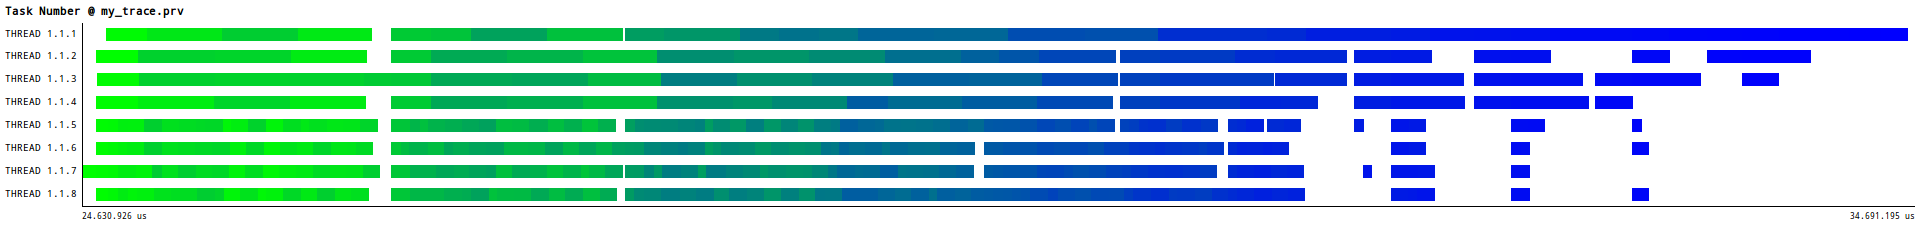
\includegraphics[width=\textwidth]{Plots/Traces/sym_8cores_task_number.png}
		\caption{OmpSs - BLIS secuencial (8 worker threads)}
	\end{subfigure}
	\begin{subfigure}{\textwidth}
   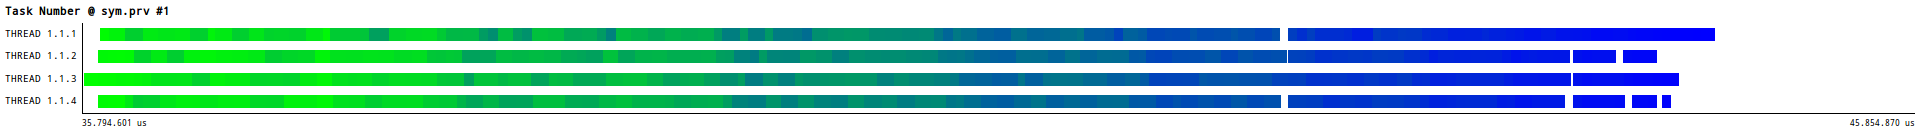
\includegraphics[width=\textwidth]{Plots/Traces/sym_task_number.png}
		\caption{OmpSs - BLIS secuencial (4 worker threads)} 
	\end{subfigure}
	\begin{subfigure}{\textwidth}
   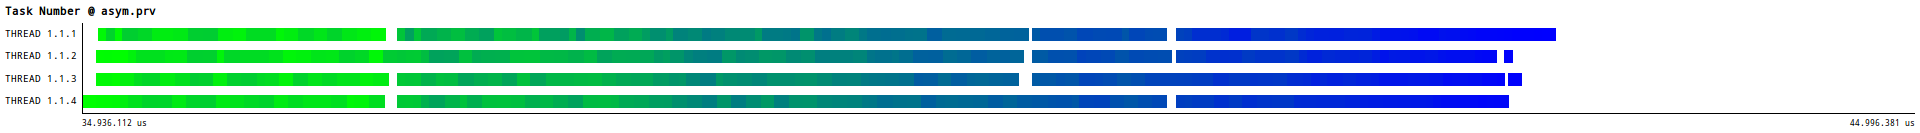
\includegraphics[width=\textwidth]{Plots/Traces/asym_task_number.png}
		\caption{OmpSs - BLIS asimétrico (4 worker threads)} 
	\end{subfigure}
	\begin{subfigure}{\textwidth}
   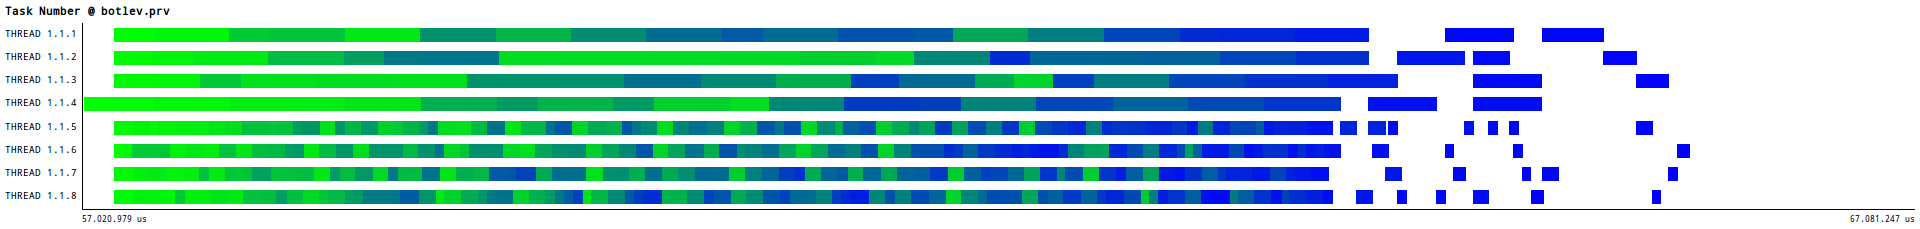
\includegraphics[width=\textwidth]{Plots/Traces/botlev_task_number.png}
		\caption{Botlev-OmpSs - BLIS secuencial (8 worker threads, 4+4)} 
	\end{subfigure}
	\caption[Orden de ejecución de tareas para las tres configuraciones estudiadas sobre la factorización de Cholesky ({\tt n}~=~6,144, {\tt b}~=~448).]{Orden de ejecución de tareas para las tres configuraciones estudiadas sobre la factorización de Cholesky
({\tt n}~=~6,144, {\tt b}~=~448). En las trazas, las tareas se ordenan según su orden de aparición
en el código secuencial, y son mostradas usando un gradiente de color, correspondiendo el color verde claro a tareas
	tempranas, y azul oscuro a tareas tardías.}
\label{fig:traces_task_number}
\end{figure}

\begin{table}
\centering
	\caption[Porcentaje de tiempo por \wt en estado {\tt idle} o {\tt running} para distintas configuraciones de planificador para la factorización de Cholesky ({\tt n}~=~6,144, {\tt b}~=~448).]
	{Porcentaje de tiempo por \wt en estado {\tt idle} o {\tt running} para distintas configuraciones de planificador para la factorización de Cholesky
({\tt n}~=~6,144, {\tt b}~=~448).
	Nótese que {\sc wt 0} es el hilo principal, y por tanto nunca permanece en estado {\tt idle} dadas las características de OmpSs; 
	para él, el resto del tiempo hasta el 100\% se dedica a sincronización, planificación y creación de la hebra. Para el resto de las hebras, esta cantidad
	de tiempo se considera sobrecoste de planificación ({\tt runtime overhead}).}
\label{tab:th_state}

\ra{1.2}
\ca{2pt}

\renewcommand{\fg}[1]{{#1}} 
\renewcommand{\br}[1]{{#1}} 

{\scriptsize
\begin{tabular}{crrrrrrrrr} 
   	\toprule
                 & \phantom{a} & \multicolumn{2}{c}{OmpSs - Seq. BLIS} & \phantom{ab} & \multicolumn{2}{c}{OmpSs - Asym. BLIS} & \phantom{ab} & \multicolumn{2}{c}{Botlev-OmpSs - Seq. BLIS} \\ 
                 & \phantom{a} & \multicolumn{2}{c}{(4 worker threads)} & \phantom{ab} & \multicolumn{2}{c}{(4 worker threads)} & \phantom{ab} & \multicolumn{2}{c}{(8 worker threads, 4+4)} \\ 
                 %& \phantom{a} & \multicolumn{4}{c}{OmpSs - Seq. BLIS} & \phantom{ab} & \multicolumn{4}{c}{OmpSs - Asym. BLIS} & \phantom{ab} & \multicolumn{4}{c}{Botlev-OmpSs - Seq. BLIS} \\ 
                 %& \phantom{a} & \multicolumn{4}{c}{(4 worker threads)} & \phantom{ab} & \multicolumn{4}{c}{(4 worker threads)} & \phantom{ab} & \multicolumn{4}{c}{(8 worker threads, 4+4)} \\ 
                                          \cmidrule{3-4}                                         \cmidrule{6-7}                                      \cmidrule{9-10}
                       & \phantom{a} &    {\tt idle}& {\tt running}& \phantom{ab}  & {\tt idle}& {\tt running}& \phantom{ab} & {\tt idle}  & {\tt running} \\ \hline 
	 {\sc wt 0}    & \phantom{a} &    \fg{--}   & \fg{98.41}   & \phantom{ab}  & \fg{--}   & \fg{97.85}   & \phantom{ab} & \fg{--}     & \fg{86.53}    \\ \cline{3-10}
	 {\sc wt 1}    & \phantom{a} &    \br{5.59} & \fg{94.22}   & \phantom{ab}  & \fg{5.51} & \fg{94.29}   & \phantom{ab} & \fg{13.63}  & \fg{86.28}    \\ \cline{3-10}
	 {\sc wt 2}    & \phantom{a} &    \br{3.14} & \fg{96.67}   & \phantom{ab}  & \fg{5.27} & \fg{94.53}   & \phantom{ab} & \fg{13.94}  & \fg{85.98}    \\ \cline{3-10}
	 {\sc wt 3}    & \phantom{a} &    \br{5.77} & \fg{94.07}   & \phantom{ab}  & \fg{5.17} & \fg{94.62}   & \phantom{ab} & \fg{13.43}  & \fg{86.47}    \\ \cline{3-10}
	 {\sc wt 4}    & \phantom{a} &    \br{--}   & \fg{--}      & \phantom{ab}  & \fg{--}   & \fg{--}      & \phantom{ab} & \fg{19.26}  & \fg{80.51}    \\ \cline{3-10}
	 {\sc wt 5}    & \phantom{a} &    \br{--}   & \fg{--}      & \phantom{ab}  & \fg{--}   & \fg{--}      & \phantom{ab} & \fg{21.12}  & \fg{78.69}    \\ \cline{3-10}
	 {\sc wt 6}    & \phantom{a} &    \br{--}   & \fg{--}      & \phantom{ab}  & \fg{--}   & \fg{--}      & \phantom{ab} & \fg{20.84}  & \fg{78.97}    \\ \cline{3-10}
	 {\sc wt 7}    & \phantom{a} &    \br{--}   & \fg{--}      & \phantom{ab}  & \fg{--}   & \fg{--}      & \phantom{ab} & \fg{20.09}  & \fg{79.70}    \\ \bottomrule
	 %{\sc TOTAL}   & \phantom{a} &    \br{13.87} & \fg{384.31}    & \phantom{ab}  & \fg{16.97}  & \fg{379.60}    & \phantom{ab} & \fg{73.81}  & \fg{715.16}   \\ \bottomrule
	 {\sc Avg.}     & \phantom{a} &    \br{4.84} & \fg{95.89}    & \phantom{ab} & \fg{5.32} & \fg{94.90}   & \phantom{ab} & \fg{17.47}  & \fg{82.89}    \\ \bottomrule
\end{tabular}
}

\end{table}



%-- Configuraciones para emacs --
%%% Local Variables:
%%% mode: latex
%%% TeX-master: "./principal.tex"
%%% End:
